\chapter{Introduction}
% observation
There is a rapid growth in the number of available biological datasets due to
the decreasing costs of data collection. This brings opportunities for gaining
novel insights into the underlying biological mechanisms in the development and
progression of diseases such as cancer, possibly leading to the development of
new diagnostic tests or drugs for treatment. The wide range of different
biological datasets has led to the development of hundreds of software packages
and systems to explore and analyze these datasets. However, there are few
systems that are designed with the full analysis process in mind, from raw data
into interpretable and reproducible results.  While existing systems are used to
provide novel insights in diseases, there is little emphasis on reporting and
sharing detailed information about the analyses. This leads to unnecessary
difficulties when reusing known methods, and reproducing the analyses, which in
turn leads to a longer analysis process and therefore unrealized potential for
scientific insights. For clinicians, inaccurate results from improperly
developed analyses can lead to negative consequences for patient
care.\cite{roy2017standards}

% challenges
We have identified four main challenges for application developers to undertake
when building systems for analyzing and exploring biological datasets in
research and the clinic. These challenges are common for large datasets such as
high-throughput sequencing data that require long-running, deep analysis
pipelines, as well as smaller datasets, such as microarray data, that require
complex, but short-running analysis pipelines. The first challenge is managing
datasets and analysis code for use by data exploration applications and data
analysis pipelines. This includes storing all information that is valuable to a
data analyst when he or she is interpreting the data, as well as any analysis
code that can be used to analyze the data. The second challenge is to develop
data exploration applications that provide sufficient information to fully
document every step that went into the analyses up to an end result. This
includes reporting input parameters, tool versions, database versions, and
dataset versions. The third challenge is developing applications that require
the integration of disparate systems. These are often developed using different
programming languages and provide different functionality, e.g., the combination
of a web-based visualization with a \gls{gpu} accelerated statistical method,
or the integration of a remote biological database.
The final challenge is to develop applications and systems so that they can be
easily shared and reused across research institutions. 

% existing tools and approaches
As a result, there is a wealth of specialized approaches and systems to manage
and analyze modern biological data. Systems such as Galaxy\cite{galaxy} provide
simple \glspl{gui} for setting up and running analysis pipelines. However, it is
difficult to install and maintain, and less flexible for explorative analyses
where it is necessary to try out new tools and different tool
configurations.\cite{spjuth2015experiences} With R and its popular package
repository Bioconductor\cite{bioconductor}, researchers can select from a wide
range of packages to tailor their analyses. These provide specialized analysis
environments, but makes it necessary for the analyst to manually record
information about data, tools, and tool versions. Systems such as
Pachyderm\cite{pachyderm} or the \gls{cwl}\cite{commonwl} and its different
implementations, can help users with standardizing the description and sharing
of analysis pipelines.  However, many of these require complex compute
infrastructure and are too cumbersome to set up.  Shiny\cite{shiny} and
OpenCPU\cite{opencpu} provide frameworks for application developers to build
systems to interactively explore results from statistical analyses.  These are
useful for building exploration applications that integrate with statistical
analyses.  With the addition of new datasets and methods every year, it seems
that analysis of biological data requires a wide array of different tools and
systems.

% our solution
This dissertation argues that, instead, we can facilitate the development of
reproducible data analysis and exploration systems for high-throughput
biological data, through the integration of disparate systems and data sources.
In particular, we show how software container technologies together with
well-defined interfaces, configurations, and orchestration provide the necessary
foundation for these systems. This allows for easy development and sharing of
specialized analysis systems.

\glsreset{sme}

The resulting approach, which we have called \glspl{sme}, argues that
applications for analyzing and exploring biological datasets should be modeled
as a composition of individual systems and tools. We believe that the Unix
philosophy to \emph{"Do one thing and do it well"}\cite{raymond2003art}
appropriately summarizes many existing tools in bioinformatics, and we should
aim to build applications as compositions of these tools. Our \gls{sme} approach
resembles the traditional Unix-like pipelines, in combination with the
service-oriented architecture\cite{erl2005service} or the microservice
architectural style now popularized by web-scale distributed
systems.\cite{nadareishvili2016microservice}

The approach has several key advantages when implementing systems to analyze and
explore biological data:
\begin{itemize} 
    \item It enables and simplifies the development of applications that
        integrate disperate tools. 
        
    \item It enables reproducible research by packaging applications
        and tools within containerized environments. 

    \item With well-defined interfaces it is a simple task to add new components
        to a system, or modify existing ones. 
        
    \item Through software container technology it becomes a simple task to
        deploy and scale up such applications. 
\end{itemize} 

In collaboration with researchers in systems epidemiology and precision
medicine we developed a set of applications and systems necessary to organize,
analyze, and interpret their datasets. From these systems we extraplolated a set
of general design principles to form a unified approach. We evaluate this
approach through these systems using real datasets to show its viability. 

From a longer-term perspective we discuss the general patterns for implementing
reproducible data analysis systems for use in biomedical research. As more
datasets are produced every year, research will depend on the simplicity of the
systems for analyzing these, and that they provide the necessary functionality
to reproduce and share the analysis pipelines. 

\emph{Thesis statement}:
A unified development model based on software container infrastructure can
efficiently provide reproducible and easy to use environments to develop
applications for exploring and analyzing biological datasets. 

\section{Problems with Data Analysis and Exploration in Bioinformatics}
Today shell scripts are often used for building analysis pipelines in
bioinformatics. This comes from the familiarity of the shell environment and the
\gls{cli} of the different tools. However, there is a move towards using more
sophisticated approaches for analyzing biological datasets using workflow and
pipeline mangers such as Snakemake\cite{koster2012snakemake}, and the different
implementations of the \gls{cwl}\cite{cwl} such as Galaxy\cite{galaxy} and
Toil\cite{toil}. These simplify setting up and executing the analysis pipeline.
However, these tools still have their limitations, such as maintenance and tool
updates. Other programming environments and scripting languages such as Python
or R both provide a wide variety of software packages to read and process
biological datasets. Especially the package repository
Bioconductor\cite{bioconductor} provides a long list of well-maintained software
packages. Both these languages require the researchers to set up their own
analyses, but can be tailored to fit their data precisely.  For visually
exploring biological data there are a range of tools, such as
Cytoscape\cite{cytoscape} and Circos\cite{circos}, that support importing an
already-analyzed dataset to visualize and browse the data. One problem with
these are that they are decoupled from the analysis, making it difficult to
retrace the underlying analyses. 

Although there are efforts to develop tools to help researchers explore and
analyze biological datasets, they current tools have several drawbacks:

\begin{enumerate}
    \item \textbf{Standardization:} Because of the specialized nature of each
        data analysis tool, a complete system for exploring or analyze
        biological data will have to combine these. The tools provide different
        interfaces and processing data using a combination of these often
        require data wrangling. 
    \item \textbf{Decoupling:} Data exploration tools are often decoupled from
        the statistical analyses. This often makes it a difficult to document
        and retrace the analyses behind the results. 
    \item \textbf{Complexity:} 
        Analyses that start as a simple script quickly become more complex to
        maintain and develop as developers add new functionality to the
        analyses. 
        % LAB: kan stjele argumentasjon fra ADAM paperet der de kritiserer
        % "monolothic" bio applikasjoner. Eller fra Tanenbaum vs Linus.
    \item \textbf{Reusability:} Data exploration tools are often
        developed as a single specialized application, making it difficult to
        reuse parts of the application for other analyses or datasets. This
        leads to duplicate development effort and abandoned projects. 
    \item \textbf{Reproducibility:} While there are tools for analyzing most
        data types today, these require the analyst to manually record versions,
        input parameters, and reference databases. This makes analysis results
        difficult to reproduce because of the large number of variables that may
        impact the results. 
\end{enumerate} 

Because of these drawbacks, a approach for unifying reproducible data analysis
and exploration systems would reduce the time-to-interpretation of biological
datasets significantly. 

\section{\acrfullpl{sme}} 
In collaboration with researchers in systems epidemiology and biology we have
developed an approach for designing applications for three specific use cases.
The first is to manage and standardize the analysis of datasets from a large
population-based cohort, \gls{nowac}.\cite{nowac}. The second is to enable
interactive exploration of these datasets.  The final use case is to develop
pipelines for analyzing sequencing datasets for use in a precision medicine
setting.  Although these use cases require widely different systems with
different requirements, the applications share common design patterns. Figure
\ref{overview-fig} shows the applications we have developed and the underlying
systems. 

\begin{figure}
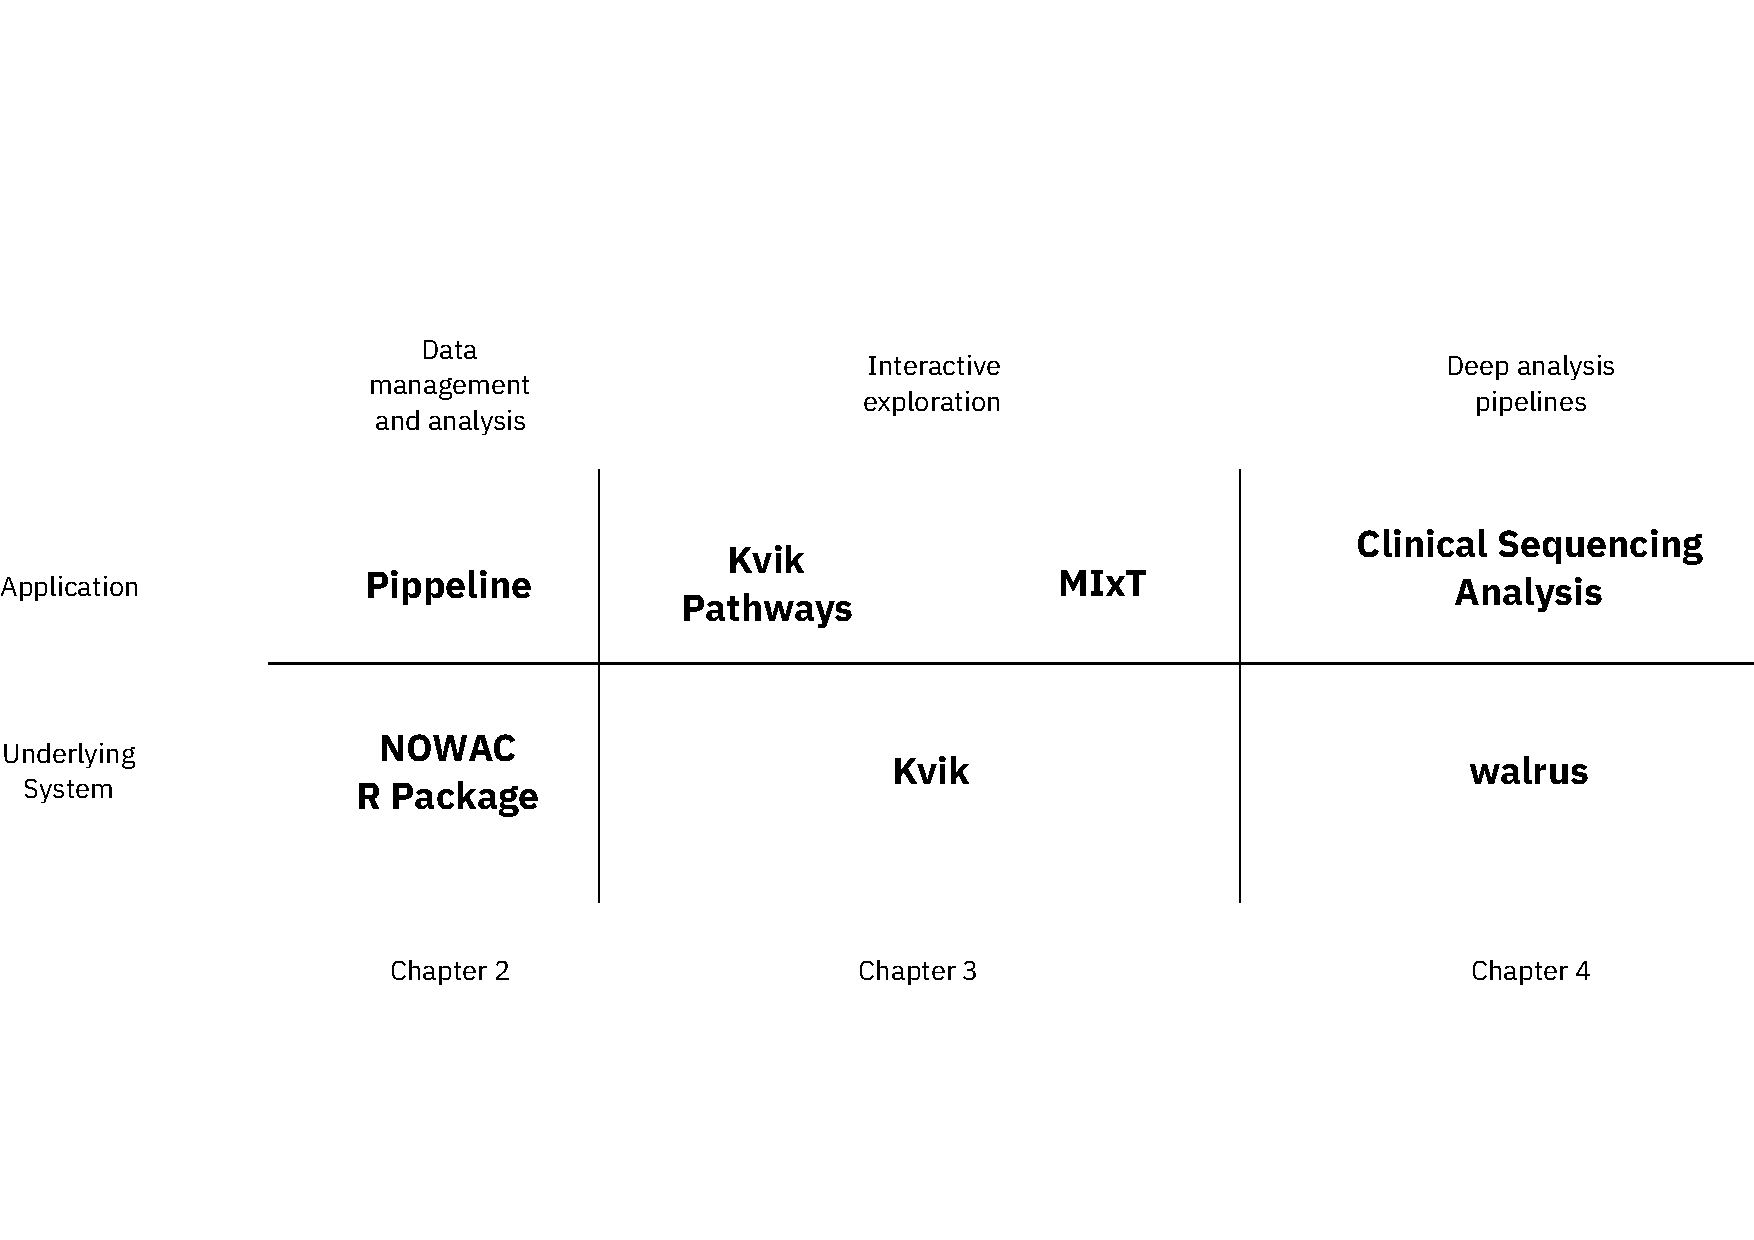
\includegraphics[width=\textwidth]{figures/all-systems.pdf}
    \caption{The applications and their underlying systems discussed in this
    thesis.} 
    \label{overview-fig}
\end{figure} 


We discuss how the approach is suitable for different use cases before
highlighting why it is suitable for all of them. Figure \ref{overview-full}
shows the three different use cases and one such \gls{sme}. We can use it in
both data exploration applications, analysis pipelines, and for building data
management systems.

\begin{figure}
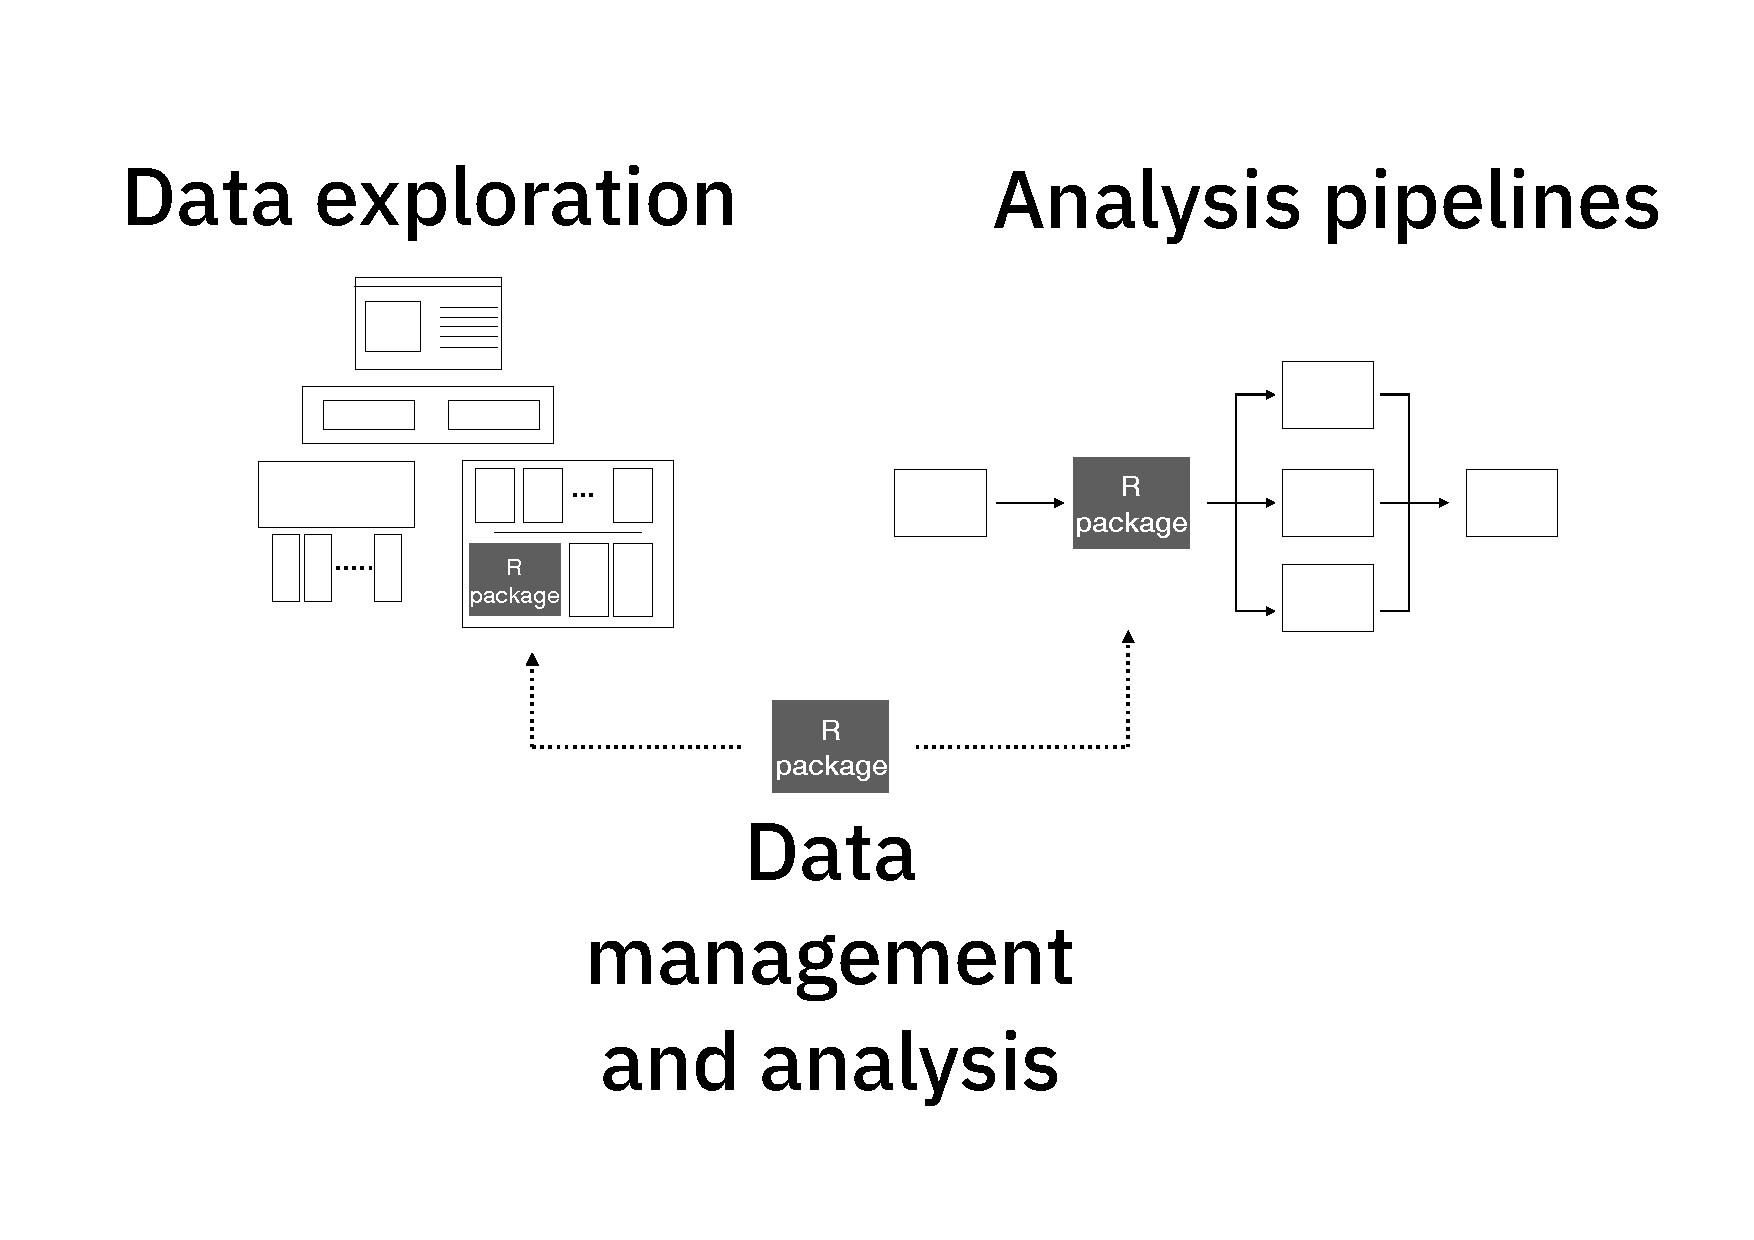
\includegraphics[width=\textwidth]{figures/overview-full.pdf}
    \caption{An illustration of how we envision the \gls{sme} approach in data
    management systems, data exploration applications and analysis pipelines. In
    this example we reuse an R package for all use cases.}
    \label{overview-full}
\end{figure} 

\subsection{Data management and analysis} 
Modern epidemiological studies integrate traditional questionnaire data with
information from public registries and biological datasets. These often span
multiple biological levels, i.e., different data types and collection sites.
While traditional survey based datasets require few specialized analysis tools
because of the relatively simple nature of the data, biological datasets require
specialized tools for reading, analyzing, and interpreting the data. Package
repositories such as Bioconductor\cite{bioconductor} provide a wealth of
packages for analyzing these datasets. These packages typically provide analysis
tools, example data, and comprehensive documentation. While the analysis code
can be shared within projects, the datasets are often stored in in-house
databases or shared file systems with specialized permissions. Together the
packages and datasets form building blocks that researchers can develop their
analyses on top of. They can compose their analyses using packages that fit
their specific needs. The analysis code in the \gls{nowac} study may constitute
such a building block. Therefore, we combined the datasets from the \gls{nowac}
cohort with documentation, analysis scripts, and integration with registry
datasets, into a single package.  This approach simplifies the researcher's
first steps in the analysis of the different data in our study. On top of the
\gls{nowac} package we then implemented a user-friendly preprocessing pipelining
tool named Pippeline. 

Inspired by the ecosystem of packages in the R programming language we
implemented our approach as the \gls{nowac} R package. Users simply install the
package and get access to documentation, datasets, and utility functions for
analyzing datasets related to their area of research. We use version
control for both code and the data, making it possible to track changes over
time as the research study evolves. Pippeline is a web-based interface for
running the standardized preprocessing steps before analyzing gene expression
datasets in the \gls{nowac} cohort. 

\subsection{Interactive Data Exploration Applications}
The final results from an analysis pipeline require researchers to investigate
and evaluate the final output. In addition, it may be useful to explore the
analysis parameters and re-run parts of the analyses. 
As with analysis pipelines, there are complete exploration tools as
well as software libraries to develop custom applications for exploration of
analysis results. The tools often require users to import already analyzed
datasets but provide interactive visualizations and point-and-click interfaces
to explore the data. Users with programming knowledge can use the wealth of
software packages for visualization within languages such as R or Python.
Frameworks such as BioJS\cite{gomez2013biojs} now provide developers with tools
to develop web applications for exploring biological datasets. It is apparent
that 
these types of systems also consist of multiple smaller components that
together can be orchestrated into a single application. These applications
typically include of three major parts:
\begin{enumerate*}[label=(\roman*)]
    \item data visualization;
    \item integration with statistical analyses and datasets; and 
    \item integration with online databases
\end{enumerate*}. 
While each of these are specialized for each type of data exploration
application, they share components that can be reused across different types of
applications. 

To facilitate the integration with statistical analyses and datasets, we wrote
an interface to the R programming language, that would allow us to interface
with the wealth of existing software packages, e.g.,  the \gls{nowac} package,
for biological data analyses from a point-and-click application. New data
exploration applications could access analyses directly through this interface,
removing the previous decoupling between the two. We followed the same approach
to integrate with online databases. We could standardize the interface from the
applications to the different databases, and implement an application on top of
these. 

We implemented all components as a part of \emph{Kvik}, a collection of packages
to develop new data exploration applications.\cite{fjukstad2015kvik} Kvik allows
applications written in any modern programming language to interface with the
wealth of bioinformatics packages in the R programming language, as well as
information available through online databases. To provide reproducible
execution environments we packaged these interfaces into  software containers
that can be easily deployed and shared.  We have used Kvik to develop the
\gls{mixt} system\cite{fjukstad2017building} for exploring and comparing
transcriptional profiles from blood and tumor samples in breast cancer patients,
in addition to applications for exploring biological
pathways\cite{fjukstad2015kvik}. 

\subsection{Deep Analysis Pipelines} 
Analysis of high-throughput sequencing datasets requires deep analysis pipelines
with many steps that transform raw data into interpretable
results.\cite{diao2015building} There are many tools available that
perform the different processing steps, written in a wide range of programming
languages. The tools and their dependencies, can be difficult to install, and
they require users to correctly manage a range of input parameters that affects
the output results. With software container technology it is a simple task for
developers to share container images with analysis tools pre-installed. Then, by
designing a text-based specification for the analyses, we can orchestrate the
execution of an entire analysis pipeline and record the flow of data through the
pipeline. As with the previous use case, we develop an analysis pipeline by
composing smaller entities, or tools, into a complete pipeline. 

We implemented the approach in \texttt{walrus}, a tool that lets users create
and run analysis pipelines. In addition, it tracks full provenance of the input,
intermediate, and output data, as well as tool parameters. With \texttt{walrus}
we have successfully built analysis pipelines to detect somatic mutations in
breast cancer patients, as well as an \gls{rna}-seq pipeline for comparison with
gene expression datasets. 

\subsection{Similarity} 
The above approaches for building data analysis and exploration applications
share the same design principles. In all areas we decompose the system, into
small modular entities, and package these into software containers which are
then orchestrated together. These containers are configured and communicate
using open protocols that make it possible to interface with them using any
programming language. We track the configuration of the containers and their
orchestration using software versioning systems, and provide the necessary
information to set up the system and reproduce their results.
We believe that the \gls{sme} approach is applicable to every step in the long
process from raw data collection to interpretable results, and that it makes
this process more transparent. 

\section{Systems Developed with \glspl{sme}}
In this section we outline the different systems we have built using
\glspl{sme}. We detail how we implemented \gls{sme} in the \gls{nowac} package,
\texttt{walrus}, and Kvik, and show applications that use these. 

\subsection{Data Management and Analysis} 
There is a need to standardize the preprocessing of biological datasets in the
\gls{nowac} study. With the \gls{nowac} package we could implement a
preprocessing pipeline on top of it that used its datasets and utility functions
to generate analysis-ready datasets for the researchers.  This preprocessing
pipeline called Pippeline was developed as a web application which allows the
data managers in our study to generate datasets for researchers.
The pipeline performs all necessary steps before researchers can perform their
specialized analyses. 

\subsection{Interactive Data Exploration Applications}
The first interactive data exploration application that we built was Kvik
Pathways.  It allows users to explore gene expression data from the \gls{nowac}
cohort in the context of interactive pathway maps.\cite{fjukstad2015kvik} It is
a web application that integrates with the R programming language to provide an
interface to the statistical analyses. We used Kvik Pathways to repeat the
analyses in a previous published project that compared gene expression in blood
from healthy women with high and low plasma ratios of essential fatty
acids.\cite{olsen2013plasma}

From the first application it became apparent that we could reuse parts of the
application in the implementation of later systems. In particular, the interface
to run analyses as well as the integration with the online databases could be
implemented as services, packaged into containers, and reused in the next
application that we developed. Both of these were designed and implemented in
Kvik, which could then be used and shared later. 

The second application that we built was the \gls{mixt} web application. A
system to explore and compare transcriptional profiles from blood and tumor
samples in breast cancer patients. The application is built to simplify the
exploration of results from the Matched Interactions Across Tissues (MIxT)
study. Its goal was to identify genes and pathways in the primary breast tumor
that are tightly linked to genes and pathways in the patient blood
cells.\cite{dumeaux2017interactions} The web application interfaces with the
methods implemented as an R package and integrates the results together with
information from biological databases through a simple user interface. 

A third application that we developed was a simple re-deployment of the
\gls{mixt} web application with a new dataset. In this application that we
simply replaced the R package with a new package that interfaced with different
data. All the other components are reused and highlights the flexibility of the
approach. 


\subsection{Deep Analysis Pipelines}
The first system that we built on top of \texttt{walrus} was a pipeline to
analyze a patient’s primary tumor and adjacent normal tissue, including
subsequent metastatic lesions.\cite{walrus} We packaged the necessary tools for
the analyses into software containers and wrote a pipeline description with all
the necessary data processing steps. Some steps required us to develop
specialized scripts to generate customized plots, but these were also wrapped in
a container. From the analyses we discovered, among other findings, inherited
germline mutations that are recognized to be among the top 50 mutations
associated with an increased risk of familial breast cancer. These were then
shared with the treating oncologists to aid the treatment plan. 

The second analysis pipeline we implemented was to enable comparison of a
\gls{rna}-seq dataset to microarray gene expression values collected from the
same samples.  The pipeline preprocesses the \gls{rna} dataset for all samples,
and generates transcript quantifications. Like the first pipeline, we used
existing tools together with specialized analysis scripts packaged into a
container to ensure that we could reproduce the execution environments. 

Combined these systems and applications demonstrate how small modular entities
are useful for both batch processing of datasets and interactive
applications. 

\section{Summary of Results} 
% TODO: SCREENSHOTS OF SOME APPS 
% TODO: Reproducibility in walrus results. 
% TODO: LAB: jeg savner "easy/ quickly" biten
We show the viability of our approach through real-world applications in systems
epidemiology and precision medicine. Through our \texttt{nowac} package and
Pippeline, we demonstrate its usefulness for enabling reproducible analyses of
biological datasets in a complex epidemiological study. We demonstrate its
usefulness for building interactive data exploration application, implemented in
\emph{Kvik}. We show the applicability of small modular entities in deep
analysis pipelines, as implemented in \texttt{walrus}.

We have used \texttt{walrus} to analyze a whole-exome dataset to from a sample
in the McGill Genome Quebec [MGGQ] dataset (GSE58644)\cite{tofigh2014prognostic}
to discover \glspl{snp}, genomic variants and somatic mutations. Using
\texttt{walrus} to analyze a dataset added 10\% to the runtime and doubled the
space requirements, but reduced days of compute time down to seconds when
restoring a previous pipeline configuration. 

We have used the packages in Kvik to develop a web application, MIxT
blood-tumor, for exploring and comparing transcriptional profiles from blood and
tumor samples in breast cancer patients.  In addition, we have used it to build
an application to explore gene expression data in the context of biological
pathways. We show that developing an application using a microservice approach
allows us to reduce database query times down to 90\%, and that we can provide
an interface to statistical analyses that is up to 10 times as fast as
alternative approaches. 

Together the results show that our approach, small modular entities, can be used
to enable reproducible data analysis and exploration of high-throughput
biological datasets while still providing the required performance. 

\section{List of papers} 
This section contains a list of papers along with short descriptions and my
contributions to each paper. 

\subsection*{Paper 1} 
\capstartfalse % disable table captions 
\begin{table}[H]
    \centering
    \begin{tabular}{ | l | p{8.8cm} | }
    \hline
         Title & Kvik: three-tier data exploration tools for flexible analysis
         of genomic data in epidemiological studies \\ \hline
         
         Authors & \textbf{Bjørn Fjukstad}, Karina Standahl Olsen, Mie Jareid,
         Eiliv Lund, and Lars Ailo Bongo \\ \hline
         
         Description & The initial description of Kvik, and how we used it to
         implement Kvik Pathways, a web application for browsing biologicap
         pathway maps integrated with gene expression data from the \gls{nowac}
         cohort. 
         \\ \hline
         
         Contribution & I designed, implemented, and deployed Kvik and Kvik
         Pathways. Evaluated the system and wrote the manuscript. \\ \hline
         
         Publication date & 15 March 2015 \\ \hline 

         Publication venue & F1000 \\ \hline
         
         Citation & \cite{fjukstad2015kvik} \bibentry{fjukstad2015kvik} \\
         \hline 
    \end{tabular}
    \label{p1}

\end{table}

\subsection*{Paper 2} 

% \hfill 
\begin{table}[H]

    \begin{tabular}{ | l | p{8.8cm} | }
    \hline
         Title & Building Applications For Interactive Data Exploration In
         Systems Biology. \\ \hline
         
         Authors & \textbf{Bjørn Fjukstad}, Vanessa Dumeaux, Karina
         Standahl Olsen, Michael Hallett, Eiliv Lund, and Lars Ailo Bongo.  \\
         \hline
         
         Description & Describes how we further developed the ideas from Paper 1
         into an approach that we used to build the \gls{mixt} web application. 
         \\ \hline
         
         Contribution & I designed, implemented, and deployed Kvik and the
         \gls{mixt} web application.  Evaluated the system and wrote the
         manuscript.  \\ \hline
         
         Publication date & 20 August 2017. \\ \hline  

         Publication venue & The 8th ACM Conference on Bioinformatics,
         Computational Biology, and Health Informatics (ACM BCB) August 20–23,
         2017.  \\
         \hline
         
         Citation & \cite{fjukstad2017building} \bibentry{fjukstad2017building}
         \\ \hline 
    \end{tabular}
    \label{p2}
    
\end{table}

\subsection*{Paper 3} 

% \hfill 
\begin{table}[H]
    
    \centering
    \begin{tabular}{ | l | p{8.8cm} | }
    \hline
         Title & Interactions Between the Tumor and the Blood Systemic Response
         of Breast Cancer Patients \\ \hline
         
         Authors & Vanessa Dumeaux, \textbf{Bjørn Fjukstad}, Hans E Fjosne,
         Jan-Ole Frantzen, Marit Muri Holmen, Enno Rodegerdts, Ellen
         Schlichting, Anne-Lise Børresen-Dale, Lars Ailo Bongo, Eiliv Lund,
         Michael Hallett.  \\ \hline
         
         Description & Describes the \gls{mixt} system which enables
         identification of genes and pathways in the primary tumor that are
         tightly
         linked to genes and pathways in the patient \gls{sr}. 
         \\ \hline
         
         Contribution & I designed, implemented, and deployed the \gls{mixt} web
         application.  Contributed to the writing of the manuscript.  \\ \hline
         
         Publication date & 28 September 2017. \\ \hline  

         Publication venue &  PLoS Computational Biology \\ \hline
         
         Citation & \cite{dumeaux2017interactions}
         \bibentry{dumeaux2017interactions}
         \\ \hline 
    \end{tabular}
    \label{p3}
    
    \hfill 

\subsection*{Paper 4} 

\begin{tabular}{ | l | p{8.8cm} | }
    \hline
     Title & A Review of Scalable Bioinformatics Pipelines \\ \hline
     
     Authors & \textbf{Bjørn Fjukstad}, Lars Ailo Bongo. \\ \hline
     
     Description & This review survey several scalable bioinformatics
     pipelines and compare their design and their use of underlying
     frameworks and infrastructures.      \\ \hline
     
     Contribution & I performed the literature review and wrote the manuscript.
     \\ \hline
     
     Publication date & 23 October 2017 \\ \hline  

     Publication venue & Data Science and Engineering\\ \hline
     
     Citation & \cite{fjukstad2017review} \bibentry{fjukstad2017review} \\
     \hline 
    \end{tabular}
    \label{p4}
\end{table}

\subsection*{Paper 5} 


\begin{table}[H]
    \centering
    \begin{tabular}{ | l | p{8.8cm} | }
    \hline
         Title & nsroot: Minimalist Process Isolation Tool Implemented With
         Linux Namespaces.  \\ \hline
         
         Authors & Inge Alexander Raknes, \textbf{Bjørn Fjukstad}, Lars Ailo
         Bongo. \\ \hline
         
         Description & Describes a tool for process isolation built using Linux
         namespaces.          \\ \hline
         
         Contribution & I contributed to the writing of the 
         manuscript, specifically to the literature review and related works.
         \\ \hline
         
         Publication date & 26 November 2017 \\ \hline  

         Publication venue & Norsk Informatikkonferanse 2017. \\ \hline
         
         Citation & \cite{NIK} \bibentry{NIK} \\
         \hline 
    \end{tabular}
    \label{p5}
\end{table}

\subsection*{Paper 6} 
\begin{table}[H]

    \centering
    \begin{tabular}{ | l | p{8.8cm} | }
    \hline
         Title & Reproducible Data Analysis Pipelines for Precision Medicine \\
         \hline
         
         Authors &  \textbf{Bjørn Fjukstad}, Vanessa Dumeaux, Michael Hallett,
         Lars Ailo Bongo\\ \hline
         
         Description & This paper outlines how we used the \glspl{sme} approach
         to build \texttt{walrus}. 
         \\ \hline
         
         Contribution & I designed, implemented, and performed the evaluation of
         \texttt{walrus}. I also wrote the manuscript. 
         \\ \hline
         
         Publication & Submitted for publication. Preprint available online at
         \url{biorxiv.org/content/early/2018/06/25/354811} \\ \hline
         
         Citation & \cite{walrus} \bibentry{walrus} \\
         \hline 
    \end{tabular}
    \label{p7}
\end{table}

\subsection{Additional Papers}
\subsubsection*{Additional Paper 1} 


% force the goddamn additional paper tables to the top of the page. 
% Fuck you Leslie. 
\raggedbottom

\begin{table}[H]
    \centering
    \begin{tabular}{ | l | p{8.8cm} | }
    \hline
         Title & Transcription factor PAX6 as a novel prognostic factor and
         putative tumour suppressor in non-small cell lung cancer \\ \hline
         
         Authors & Yury Kiselev, Sigve Andersen, Charles Johannessen, 
         \textbf{Bjørn Fjukstad}, Karina Standahl Olsen, Helge Stenvold, Samer
         Al-Saad, Tom Dønnem, Elin Richardsen, Roy M Bremnes, and Lill-Tove
         Rasmussen Busund.\\ \hline
         
         Description & This paper explores the possibility of using the PAX6
         transcription factor as a prognostic marker in non-small cell lung
         cancer. 
         \\ \hline
         
         Contribution & I did the analyses to explore association between PAX6
         gene expression and PAX6 target genes. 
         \\ \hline
         
         Publication date & 22 March 2018 \\ \hline  

         Publication venue & Scientific Reports\\ \hline
         
         Citation & \cite{kiselev2018transcription}
         \bibentry{kiselev2018transcription} \\
         \hline 
    \end{tabular}
    \label{adp1}
\end{table}

\subsubsection*{Additional Paper 2} 
\begin{table}[H]
    \centering
    \begin{tabular}{ | l | p{8.8cm} | }
    \hline
         Title & Low-Cost Programmable Air Quality Sensor Kits in Science
         Education \\ \hline
         
         Authors & \textbf{Bjørn Fjukstad}, Nina Angelvik, Maria Wulff Hauglann,
         Joachim Sveia Knutsen, Morten Grønnesby, Hedinn Gunhildrud, and Lars
         Ailo Bongo.  \\ \hline
         
         Description & In this paper we describe a science education project for
         students in upper-secondary schools.  Students build and program their
         own air quality sensor kits to collect air quality data.  We used the
         same \gls{sme} approach to develop the \url{airbit.uit.no} web
         application where students can upload and explore their collected data. 
         \\ \hline
         
         Contribution & I designed the project, implemented the web application,
         and wrote the paper. 
         \\ \hline
         
         Publication date & 22 February 2018 \\ \hline  

         Publication venue & The 49th ACM Technical Symposium on Computer
         Science Education \\ \hline
         
         Citation & \cite{fjukstad2018low}
         \bibentry{fjukstad2018low} \\
         \hline 
    \end{tabular}
    \label{adp2}
\end{table}

% move table to top of page hack
\makeatletter
\afterpage{\global\let\@textbottom\relax \global\let\@texttop\relax}



% \subsection*{Paper 8} 
% \begin{table}[H]
% 
%     \centering
%     \begin{tabular}{ | l | p{9.5cm} | }
%     \hline
%          Title & Standardizing Data Analysis in a Complex Population-Based
%          Epidemiological Study \\
%          \hline
%          
%          Authors & \textbf{Bjørn Fjukstad}, Nikita Shvetsov, Hege Bøvelstad,
%          Till Halbach, Einar Holsbø, Eiliv Lund, Lars Ailo Bongo.
%            \\ \hline
%          
%          Description & This paper outlines our efforts to standardize the
%          data analysis and management systems in the \gls{nowac} study. It
%          describes the \gls{nowac} package and the preprocessing pipeline,
%          called Pippeline.
%          \\ \hline
%          
%          Contribution & Design and implementation of the \gls{nowac} package. 
%          Contributed to writing of the manuscript. 
%          \\ \hline
%          
%          Publication date & TBA \\ \hline  
% 
%          Publication venue & TBA \\ \hline
%          
%          Citation & \cite{pippeline} \bibentry{pippeline} \\
%          \hline 
%     \end{tabular}
%     \label{p8}
% \end{table}

% Husk historien: Fra rå data gjennom komplekse analyse pipeliner og helt til
% forskere kan svømme rundt i resultatene. 

\section{Dissertation Plan} 
This thesis is organized as follows. Chapter 2 describes the characteristics of
state-of-the-art biological datasets in systems epidemiology and how we have
developed an approach to analyze these. 
In Chapter 3 we describe how we used the same ideas and model to develop
applications for interactively exploring results from statistical analyses.
Chapter 4 explores how we can develop analysis pipelines for high-throughput
sequencing datasets in precision medicine. It describes in detail how we use a
container centric development model to build a tool, walrus, to develop and
execute these pipelines.
Finally, Chapter 5 concludes the work and discusses future directions. 

